\section{Visão geral de problemas de otimização}

Os problemas de otimização, também conhecidos como problemas de programação matemática, envolvem encontrar um ou mais valores ótimos para um conjunto de expressões matemáticas. Um ótimo pode ser um valor que maximiza uma expressão (máximo) ou que minimiza uma expressão (mínimo). Quando o problema em questão envolve a determinação de máximos, chama-se problema de maximização -- ou minimização, no caso de mínimos.

Em cursos de cálculo, os problemas de otimização propostos costumam ser relativamente simples. Geralmente, apresenta-se uma \emph{função objetivo} de uma variável e pede-se que seja maximizada ou minimizada. Neste caso, a resolução costuma ser simples, de acordo com o seguinte passo a passo \cite{STEWART2016}:

\begin{enumerate}
    \item Dada a função a otimizar, $f(x)$, determinar as derivadas $f'(x)$ e $f''(x)$.
    \item Encontrar os zeros de $f'(x)$, conhecidos como pontos críticos de $f(x)$.
    \item Sejam $x_1,\dots,x_n$ os pontos críticos de $f$. Calcular $y_k = f''(x_k) \forall k \in \{1,\dots,n\}$.
    \item Se o problema for de maximização, os pontos de máximo são os $x_k$ para os quais $y_k < 0$. Se o problema for de minimização, os pontos de mínimo são os $x_k$ para os quais $y_k > 0$.
\end{enumerate}

Nota-se que podem existir vários pontos máximos e mínimos. É possível, portanto, que $x_a$ e $x_b$ sejam ambos pontos de máximo, com $x_a > x_b$. Isso significa que $x_a$ e $x_b$ resultam nos maiores valores de $f(x)$ em intervalos específicos da função. A \cref{fig:maxmin exemplo} exemplifica graficamente esta questão. A função ilustrada contém dois pontos de máximo e um ponto de mínimo. Em relação aos pontos de máximo, o ponto à esquerda está claramente acima de todos os outros pontos da função. Por esta razão, diz-se que este é um máximo \emph{global} da função. Já o ponto à direita, por ser máximo de um intervalo reduzido do domínio da função, é chamado de máximo \emph{local}. Por fim, apesar de a função ter um único ponto de mínimo, este não é um mínimo global, dado que $x \to -\infty \Rightarrow f(x) \to -\infty$ e $x \to \infty \Rightarrow f(x) \to -\infty$. Ou seja, é possível que um problema não tenha ótimos globais.

\begin{figure}[ht]
    \centering
    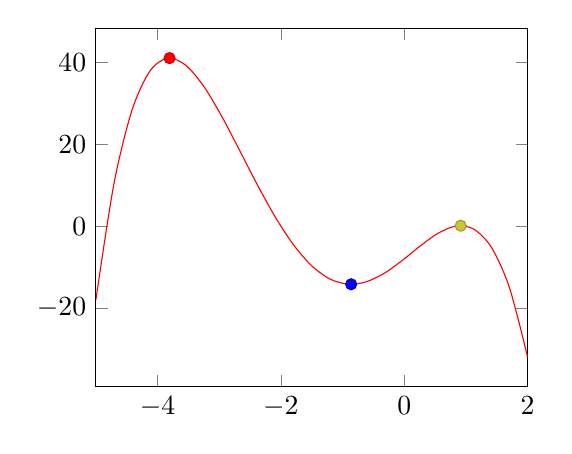
\begin{tikzpicture}
        \begin{axis}[scale=0.8, xmin=-5, xmax=2]
            \addplot[color=red,smooth,domain=-5:2]{-x^4-5*x^3+2*x^2+12*x-8};
            \addplot[scatter, only marks]table{
                x y
                -3.80562 41.12727 
                -0.86048 -14.20753
                0.91611 0.12322 
            };
        \end{axis}
    \end{tikzpicture}
    \caption{Pontos de máximo e mínimo de uma função}
    \label{fig:maxmin exemplo}
\end{figure}

Problemas reais de otimização costumam ser mais complexos do que isso. Um exemplo clássico considera uma empresa que precisa decidir qual quantidade de cada produto produzir para maximizar seu lucro \cite{ZHANG2020}. Neste caso, não faz sentido qualquer solução onde a quantidade de determinado produto seja $< 0$ e, portanto, é necessário impor \emph{restrições} ao modelo do problema. Também é importante observar que $n$ produtos diferentes representam $n$ quantidades diferentes que devem ser definidas para resolver o problema de otimização. Ou seja, a função objetivo é uma função de $n$ variáveis.

Todos os fatores apresentados até aqui conspiram contra a resolução do problema por métodos manuais. De fato, a maioria dos problemas de otimização tem sua resolução feita por métodos computacionais, como o método simplex \cite{BAZARAA2010,BERTSIMAS1997}, comumente utilizado para resolver problemas de programação linear -- ou seja, problemas cuja função objetivo e cujas restrições são lineares. Entretanto, mesmo o simplex tem suas limitações. Em trabalho de iniciação científica realizado sobre este método \cite{CENTENARO2023}, constatou-se que os principais fatores que dificultam a resolução de problemas são:

\begin{itemize}
    \item Grande número de restrições: A resolução de problemas de otimização por meio do método simplex é baseada numa interpretação geométrica das restrições impostas sobre o modelo. Assim, quanto maior o número de restrições, mais complexa é a geometria do problema, o que pode resultar em mais passos para resolvê-lo.
    \item Restrições inteiras: Pode-se querer que certas variáveis do problema sejam números naturais, inteiros ou binários. Neste caso, o método simplex deixa de funcionar, e costumam-se aplicar métodos de otimização inteira como o \emph{branch-and-bound}, que cria uma árvore de sub-problemas que podem ser resolvidos usando o simplex. Tal árvore pode crescer rapidamente, executando o simplex várias vezes, sem a garantia de convergência para um valor ótimo em cada galho.
\end{itemize}

No caso de problemas não-lineares, a otimização é ainda mais difícil, pois existem vários métodos diferentes, que têm vantagens e desvantagens dependentes de características matemáticas específicas de cada problema \cite{RIBEIRO2013}.

\subsection{Heurísticas para otimização}

Métodos como o simplex são ditos \emph{exatos}, pois são feitos para retornar valores ótimos de fato. Contudo, como arguido anteriormente, problemas muito complexos podem ter uma resolução exata muito lenta. Por este motivo, muitos problemas práticos de otimização são resolvidos por \emph{heurísticas}. As heurísticas são métodos que visam simplificar modelos de otimização de modo a resolvê-los mais rapidamente. Frequentemente, isso resulta em soluções não-ótimas, de onde resulta que uma ``boa'' heurística deve ser rápida e, ao mesmo tempo, conduzir a valores próximos do ótimo. Convém observar que heurísticas costumam ser separadas em duas categorias, que são apresentadas a seguir.

\subsubsection*{Heurísticas convencionais}

Heurísticas convencionais são projetadas para resolver problemas específicos. Um exemplo é a heurística de \textcite{GEORGE1980} para carregamento de contêineres com itens cuboides. Para concluir este objetivo, a heurística fatia o contêiner em vários volumes cuboides menores e aplica uma série de procedimentos para preenchê-los. Uma heurística popular para resolver problemas de roteamento de veículos é o método \emph{nearest neighbor} \cite{LIU2023}, que consiste em construir rotas ponto a ponto, sempre escolhendo o ponto não visitado menos distante como próximo ponto do trajeto. Como estas heurísticas criam soluções do zero, são chamadas de heurísticas \emph{construtivas}. Geralmente, heurísticas construtivas são aperfeiçoadas por heurísticas \emph{de melhoria}, que costumam introduzir alterações aleatórias nas soluções geradas em busca de soluções melhores.

\subsubsection*{Meta-heurísticas}

Em geral, as meta-heurísticas operam em uma de duas maneiras. No primeiro caso, o método extrai informações específicas sobre o problema e em seguida escolhe uma heurística que parece mais apropriada para resolvê-lo. No segundo caso, a meta-heurística é baseada em processos naturais que podem ser abstraídos para resolver uma vasta gama de problemas. É possível citar métodos como recozimento simulado (\emph{simulated annealing}), algoritmos genéticos, colônia de formigas, busca tabu, entre outros. Como exemplo, o primeiro procedimento citado é descrito a seguir.

O recozimento simulado é baseado numa técnica metalúrgica de remoção de tensões internas provenientes de deformidades na estrutura cristalina de um metal. De acordo com \textcite{DELAHAYE2019}, o processo consiste em aquecer o metal até seu ponto de fusão. Neste estado, os átomos que constituem o metal estão dispersos aleatoriamente no espaço. Em seguida, inicia-se um processo lento de resfriamento, após o qual os átomos tendem a se distribuir de forma homogênea, de modo a minimizar a energia retida na estrutura cristalina.

Para imitar os procedimentos descritos, o recozimento simulado precisa de uma função ($f$) capaz de avaliar soluções para o problema especificado, o que é análogo a medir a energia da estrutura cristalina do metal. No lugar de tempo, usa-se o número de iterações do método ($k$) para ``cronometrar'' o processo. Além disso, introduz-se um parâmetro de temperatura ($T$) que é reduzido a cada iteração. O método costuma se resumir aos seguintes passos:

\begin{enumerate}
    \item Gerar uma solução inicial e inicializar os parâmetros.
    \item Gerar uma nova solução, fazendo modificações na solução atual.
    \item Comparar a solução nova à atual usando a função $f$.
    \item   \begin{enumerate}
                \item Se a solução nova for melhor do que a atual, ela passa a ser a solução atual.
                \item Se a solução nova for pior do que a atual, utiliza-se um método aleatório para determinar se ela deve substituir a atual, de modo que as chances sejam maiores quando a temperatura $T$ for maior.
            \end{enumerate}
    \item Reduzir a temperatura $T$.
    \item Se a temperatura $T$ tiver chegado ao seu valor mínimo, terminar o algoritmo e retornar a solução atual. Do contrário, voltar ao passo 2.
\end{enumerate}